\documentclass{standalone}
\usepackage[T1]{fontenc}
\usepackage[utf8]{inputenc}
\usepackage[usenames,dvipsnames]{xcolor}
\usepackage{tikz}
\usetikzlibrary{plotmarks}
\usetikzlibrary{shapes,snakes,arrows}
\begin{document}
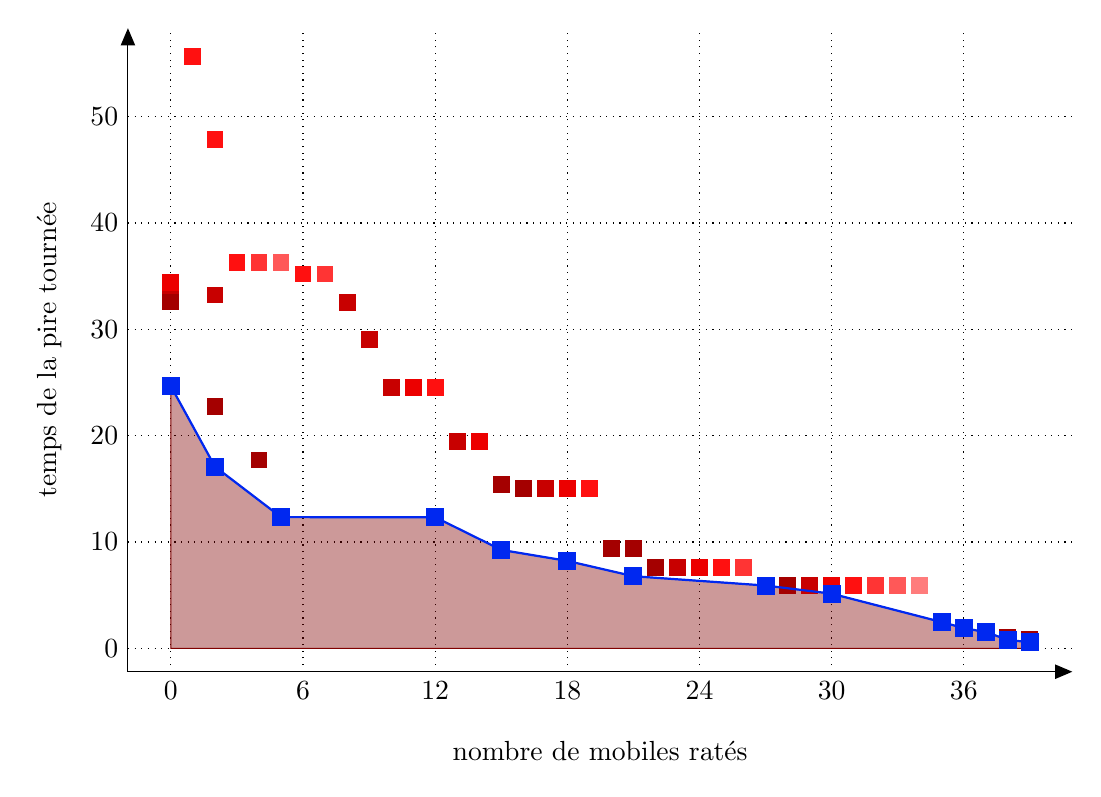
\begin{tikzpicture}[xscale=0.27972,yscale=0.135053]
\draw[xstep=6,ystep=10,thin,dotted,color=Black] (-1.95,-2.19545) grid (40.9261,58.3158);
\begin{scope}
  \clip (-1.95,-2.19545) rectangle (40.9261,58.3158);
  \definecolor{hvColor}{RGB}{128,0,0}
  \draw[color=hvColor, fill=hvColor, fill opacity=0.4] (0,0.558335) -- (0,24.6527) -- (2,17.0939) -- (5,12.3414) -- (12,12.3341) -- (15,9.2603) -- (18,8.22229) -- (21,6.78512) -- (27,5.90786) -- (30,5.14178) -- (35,2.47133) -- (36,1.90405) -- (37,1.52822) -- (38,0.807289) -- (39,0.558335) -| (39,0.558335) |- (0,0) -- cycle;
  \definecolor{pLineColor}{RGB}{164,0,0}
  \definecolor{pPointColor}{RGB}{164,0,0}
  \node[draw,color=pPointColor,fill=pPointColor, inner sep = 0pt, minimum size=2mm] at (0,32.5807) {};
  \node[draw,color=pPointColor,fill=pPointColor, inner sep = 0pt, minimum size=2mm] at (2,22.7534) {};
  \node[draw,color=pPointColor,fill=pPointColor, inner sep = 0pt, minimum size=2mm] at (4,17.7162) {};
  \node[draw,color=pPointColor,fill=pPointColor, inner sep = 0pt, minimum size=2mm] at (15,15.3923) {};
  \node[draw,color=pPointColor,fill=pPointColor, inner sep = 0pt, minimum size=2mm] at (16,15.0591) {};
  \node[draw,color=pPointColor,fill=pPointColor, inner sep = 0pt, minimum size=2mm] at (20,9.40584) {};
  \node[draw,color=pPointColor,fill=pPointColor, inner sep = 0pt, minimum size=2mm] at (21,9.3819) {};
  \node[draw,color=pPointColor,fill=pPointColor, inner sep = 0pt, minimum size=2mm] at (22,7.64461) {};
  \node[draw,color=pPointColor,fill=pPointColor, inner sep = 0pt, minimum size=2mm] at (28,5.90786) {};
  \node[draw,color=pPointColor,fill=pPointColor, inner sep = 0pt, minimum size=2mm] at (38,1.01929) {};
  \node[draw,color=pPointColor,fill=pPointColor, inner sep = 0pt, minimum size=2mm] at (39,0.807289) {};
  \definecolor{pLineColor}{RGB}{200,0,0}
  \definecolor{pPointColor}{RGB}{200,0,0}
  \node[draw,color=pPointColor,fill=pPointColor, inner sep = 0pt, minimum size=2mm] at (0,34.0791) {};
  \node[draw,color=pPointColor,fill=pPointColor, inner sep = 0pt, minimum size=2mm] at (2,33.2272) {};
  \node[draw,color=pPointColor,fill=pPointColor, inner sep = 0pt, minimum size=2mm] at (8,32.4847) {};
  \node[draw,color=pPointColor,fill=pPointColor, inner sep = 0pt, minimum size=2mm] at (9,29.0584) {};
  \node[draw,color=pPointColor,fill=pPointColor, inner sep = 0pt, minimum size=2mm] at (10,24.5615) {};
  \node[draw,color=pPointColor,fill=pPointColor, inner sep = 0pt, minimum size=2mm] at (13,19.4886) {};
  \node[draw,color=pPointColor,fill=pPointColor, inner sep = 0pt, minimum size=2mm] at (17,15.0591) {};
  \node[draw,color=pPointColor,fill=pPointColor, inner sep = 0pt, minimum size=2mm] at (23,7.64461) {};
  \node[draw,color=pPointColor,fill=pPointColor, inner sep = 0pt, minimum size=2mm] at (29,5.90786) {};
  \definecolor{pLineColor}{RGB}{236,0,0}
  \definecolor{pPointColor}{RGB}{236,0,0}
  \node[draw,color=pPointColor,fill=pPointColor, inner sep = 0pt, minimum size=2mm] at (0,34.3734) {};
  \node[draw,color=pPointColor,fill=pPointColor, inner sep = 0pt, minimum size=2mm] at (11,24.5615) {};
  \node[draw,color=pPointColor,fill=pPointColor, inner sep = 0pt, minimum size=2mm] at (14,19.4886) {};
  \node[draw,color=pPointColor,fill=pPointColor, inner sep = 0pt, minimum size=2mm] at (18,15.0591) {};
  \node[draw,color=pPointColor,fill=pPointColor, inner sep = 0pt, minimum size=2mm] at (24,7.64461) {};
  \node[draw,color=pPointColor,fill=pPointColor, inner sep = 0pt, minimum size=2mm] at (30,5.90786) {};
  \definecolor{pLineColor}{RGB}{255,16,16}
  \definecolor{pPointColor}{RGB}{255,16,16}
  \node[draw,color=pPointColor,fill=pPointColor, inner sep = 0pt, minimum size=2mm] at (1,55.634) {};
  \node[draw,color=pPointColor,fill=pPointColor, inner sep = 0pt, minimum size=2mm] at (2,47.8672) {};
  \node[draw,color=pPointColor,fill=pPointColor, inner sep = 0pt, minimum size=2mm] at (3,36.2648) {};
  \node[draw,color=pPointColor,fill=pPointColor, inner sep = 0pt, minimum size=2mm] at (6,35.2021) {};
  \node[draw,color=pPointColor,fill=pPointColor, inner sep = 0pt, minimum size=2mm] at (12,24.5615) {};
  \node[draw,color=pPointColor,fill=pPointColor, inner sep = 0pt, minimum size=2mm] at (19,15.0591) {};
  \node[draw,color=pPointColor,fill=pPointColor, inner sep = 0pt, minimum size=2mm] at (25,7.64461) {};
  \node[draw,color=pPointColor,fill=pPointColor, inner sep = 0pt, minimum size=2mm] at (31,5.90786) {};
  \definecolor{pLineColor}{RGB}{255,52,52}
  \definecolor{pPointColor}{RGB}{255,52,52}
  \node[draw,color=pPointColor,fill=pPointColor, inner sep = 0pt, minimum size=2mm] at (4,36.2648) {};
  \node[draw,color=pPointColor,fill=pPointColor, inner sep = 0pt, minimum size=2mm] at (7,35.2021) {};
  \node[draw,color=pPointColor,fill=pPointColor, inner sep = 0pt, minimum size=2mm] at (26,7.64461) {};
  \node[draw,color=pPointColor,fill=pPointColor, inner sep = 0pt, minimum size=2mm] at (32,5.90786) {};
  \definecolor{pLineColor}{RGB}{255,88,88}
  \definecolor{pPointColor}{RGB}{255,88,88}
  \node[draw,color=pPointColor,fill=pPointColor, inner sep = 0pt, minimum size=2mm] at (5,36.2648) {};
  \node[draw,color=pPointColor,fill=pPointColor, inner sep = 0pt, minimum size=2mm] at (33,5.90786) {};
  \definecolor{pLineColor}{RGB}{255,124,124}
  \definecolor{pPointColor}{RGB}{255,124,124}
  \node[draw,color=pPointColor,fill=pPointColor, inner sep = 0pt, minimum size=2mm] at (34,5.90786) {};
  \definecolor{pLineColor}{RGB}{128,0,0}
  \definecolor{pPointColor}{RGB}{0,40,240}
  \draw[thick,color=pPointColor] (0,24.6527) node[draw,color=pPointColor,fill=pPointColor, inner sep = 0pt, minimum size=2mm] {} -- (2,17.0939) node[draw,color=pPointColor,fill=pPointColor, inner sep = 0pt, minimum size=2mm] {} -- (5,12.3414) node[draw,color=pPointColor,fill=pPointColor, inner sep = 0pt, minimum size=2mm] {} -- (12,12.3341) node[draw,color=pPointColor,fill=pPointColor, inner sep = 0pt, minimum size=2mm] {} -- (15,9.2603) node[draw,color=pPointColor,fill=pPointColor, inner sep = 0pt, minimum size=2mm] {} -- (18,8.22229) node[draw,color=pPointColor,fill=pPointColor, inner sep = 0pt, minimum size=2mm] {} -- (21,6.78512) node[draw,color=pPointColor,fill=pPointColor, inner sep = 0pt, minimum size=2mm] {} -- (27,5.90786) node[draw,color=pPointColor,fill=pPointColor, inner sep = 0pt, minimum size=2mm] {} -- (30,5.14178) node[draw,color=pPointColor,fill=pPointColor, inner sep = 0pt, minimum size=2mm] {} -- (35,2.47133) node[draw,color=pPointColor,fill=pPointColor, inner sep = 0pt, minimum size=2mm] {} -- (36,1.90405) node[draw,color=pPointColor,fill=pPointColor, inner sep = 0pt, minimum size=2mm] {} -- (37,1.52822) node[draw,color=pPointColor,fill=pPointColor, inner sep = 0pt, minimum size=2mm] {} -- (38,0.807289) node[draw,color=pPointColor,fill=pPointColor, inner sep = 0pt, minimum size=2mm] {} -- (39,0.558335) node[draw,color=pPointColor,fill=pPointColor, inner sep = 0pt, minimum size=2mm] {};
\end{scope}
\draw[->,>=triangle 45] (-1.95,-2.19545) -- coordinate (x axis mid) (40.9261,-2.19545);
\node[below=1cm,anchor=center] at (x axis mid) {nombre de mobiles ratés};
\foreach \x in {0,6,12,18,24,30,36}
  \draw (\x,-2.19545) -- (\x,-2.19545) node[anchor=north] {\x};
\draw[->,>=triangle 45] (-1.95,-2.19545) -- coordinate (y axis mid) (-1.95,58.3158);
\node[left=1cm,rotate=90,anchor=center] at (y axis mid) {temps de la pire tournée};
\foreach \y in {0,10,20,30,40,50}
  \draw (-1.95,\y) -- (-1.95,\y) node[anchor=east] {\y};
\end{tikzpicture}
\end{document}
